\newpage
\newgeometry{left=3cm,right=1.5cm,top=1cm,bottom=1.5cm}
\appendix
\begin{landscape}
\begin{center}
    \bfseries\LARGE Apéndice \par
\end{center}

% Insertar imagen de la simulación de la etapa de carga
\begin{figure}[hbt]
    \centering
    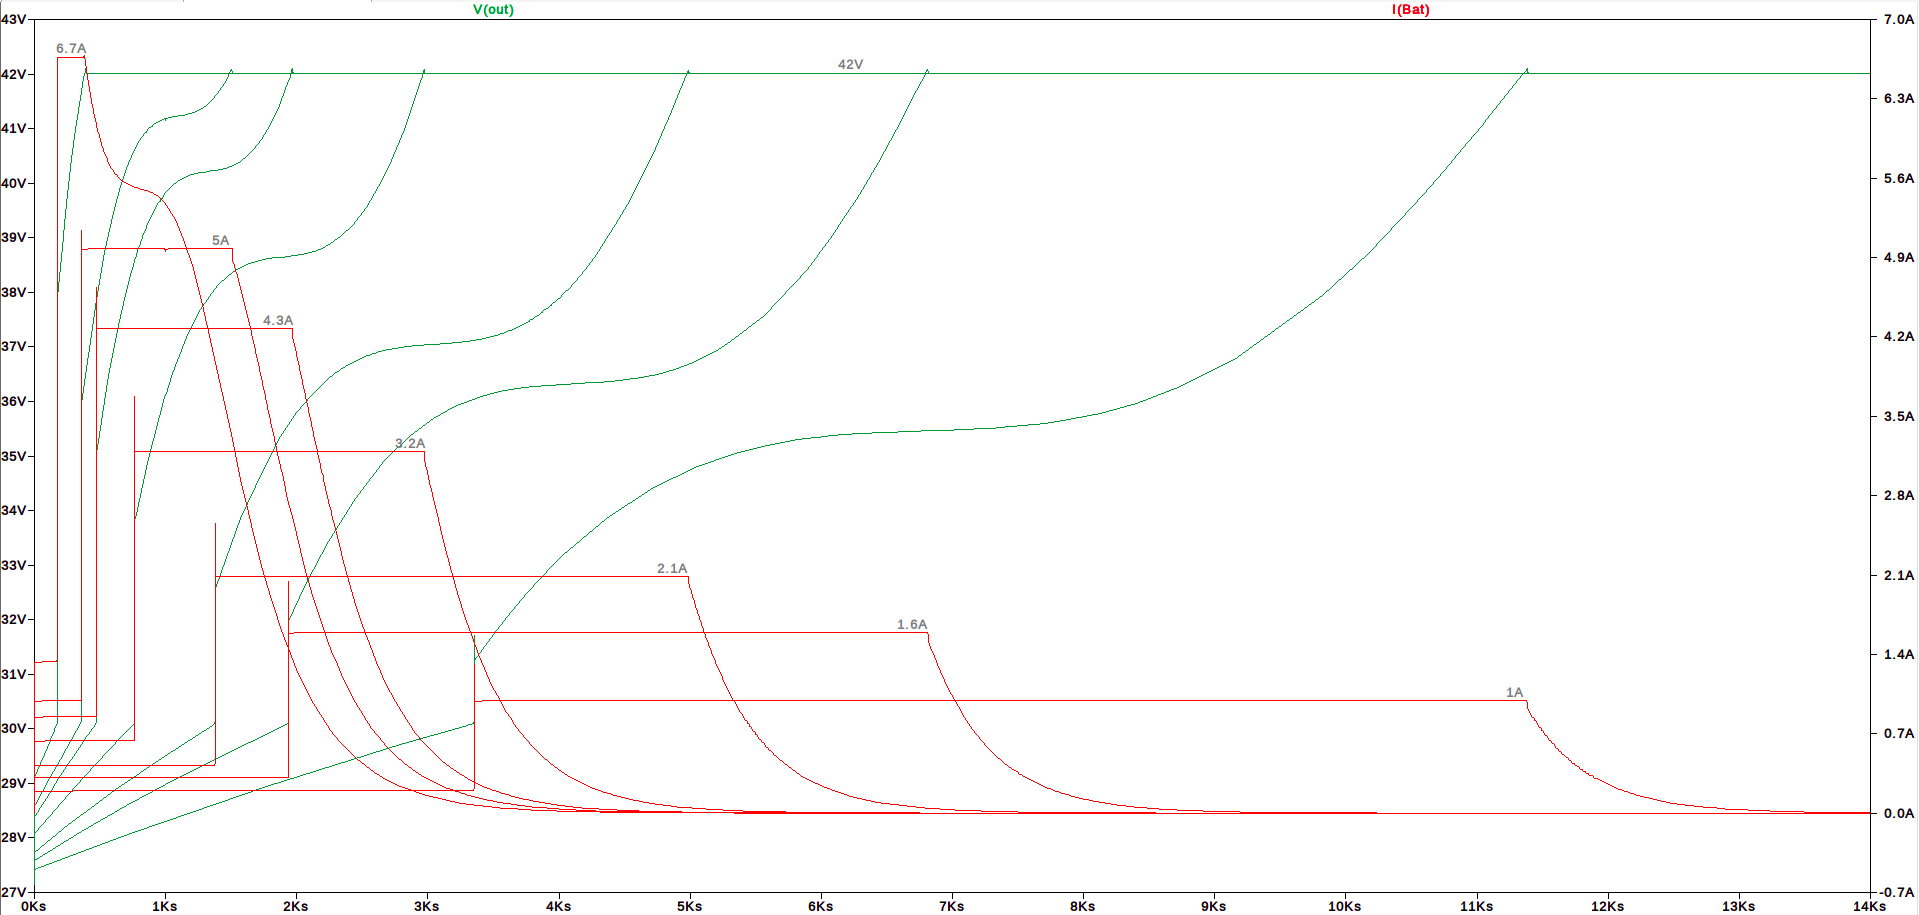
\includegraphics[width=\linewidth]{images/carga_completa_step.png}
    \caption{Simulación de las etapas de carga para todos los modos de corriente}
    \label{fig:simulacion_carga}
\end{figure}
    
\begin{figure}[hbt]
    \centering
    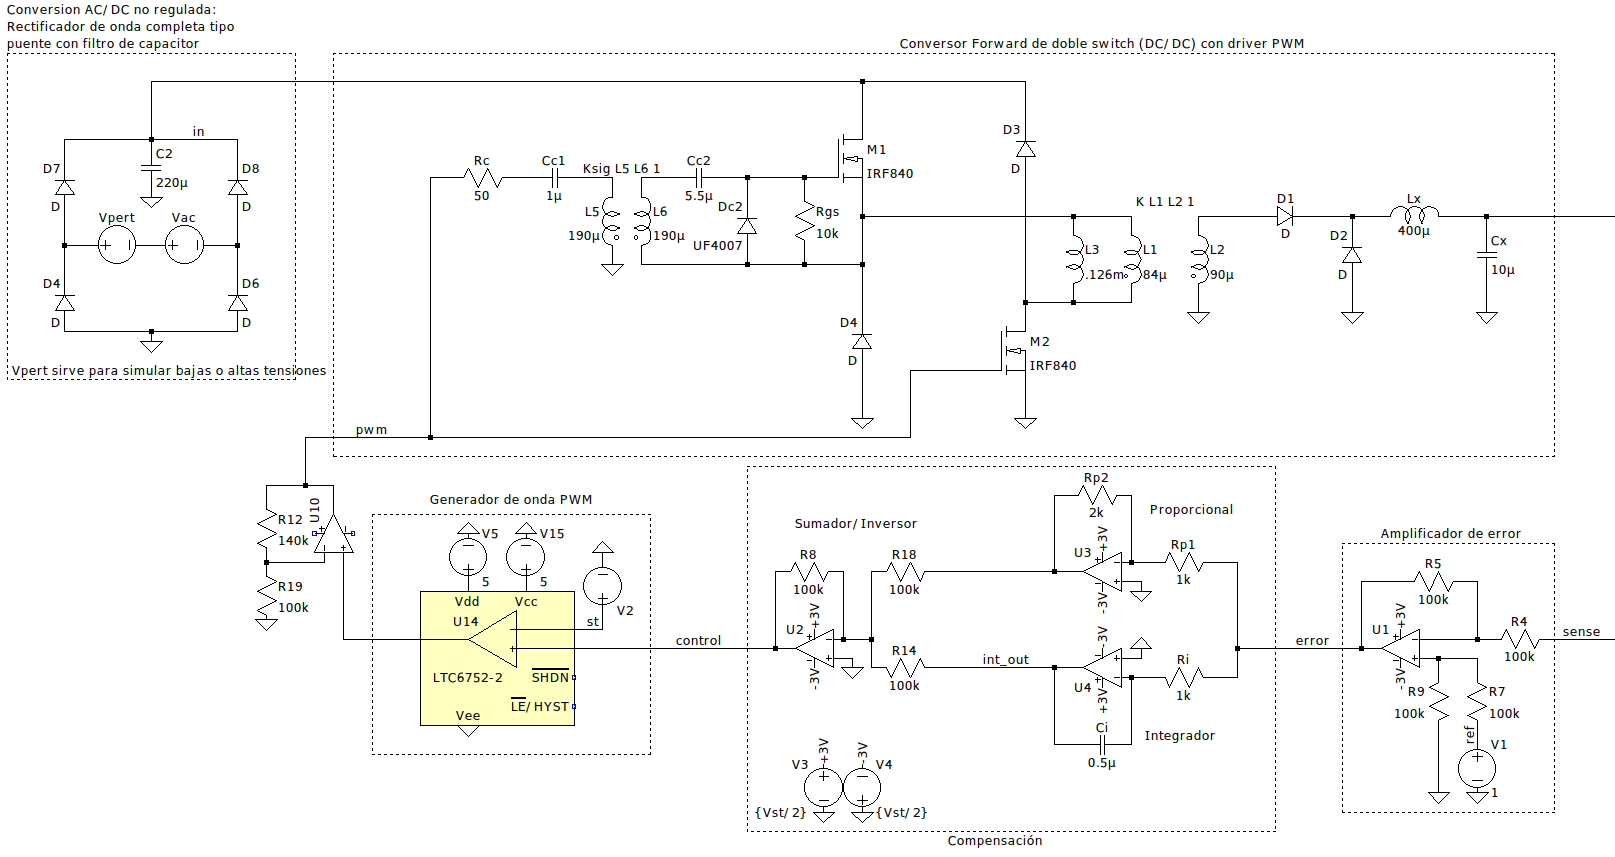
\includegraphics[width=\linewidth]{images/sim-full-1.png}
    \caption{Circuito simulado en LTspice. Se separa cada bloque con línea punteada. Se muestra el recitificador de entrada, el convertidor DC-DC y parte del circuito de control.}
    \label{fig:sim-full-1}
\end{figure}

\begin{figure}[hbt]
    \centering
    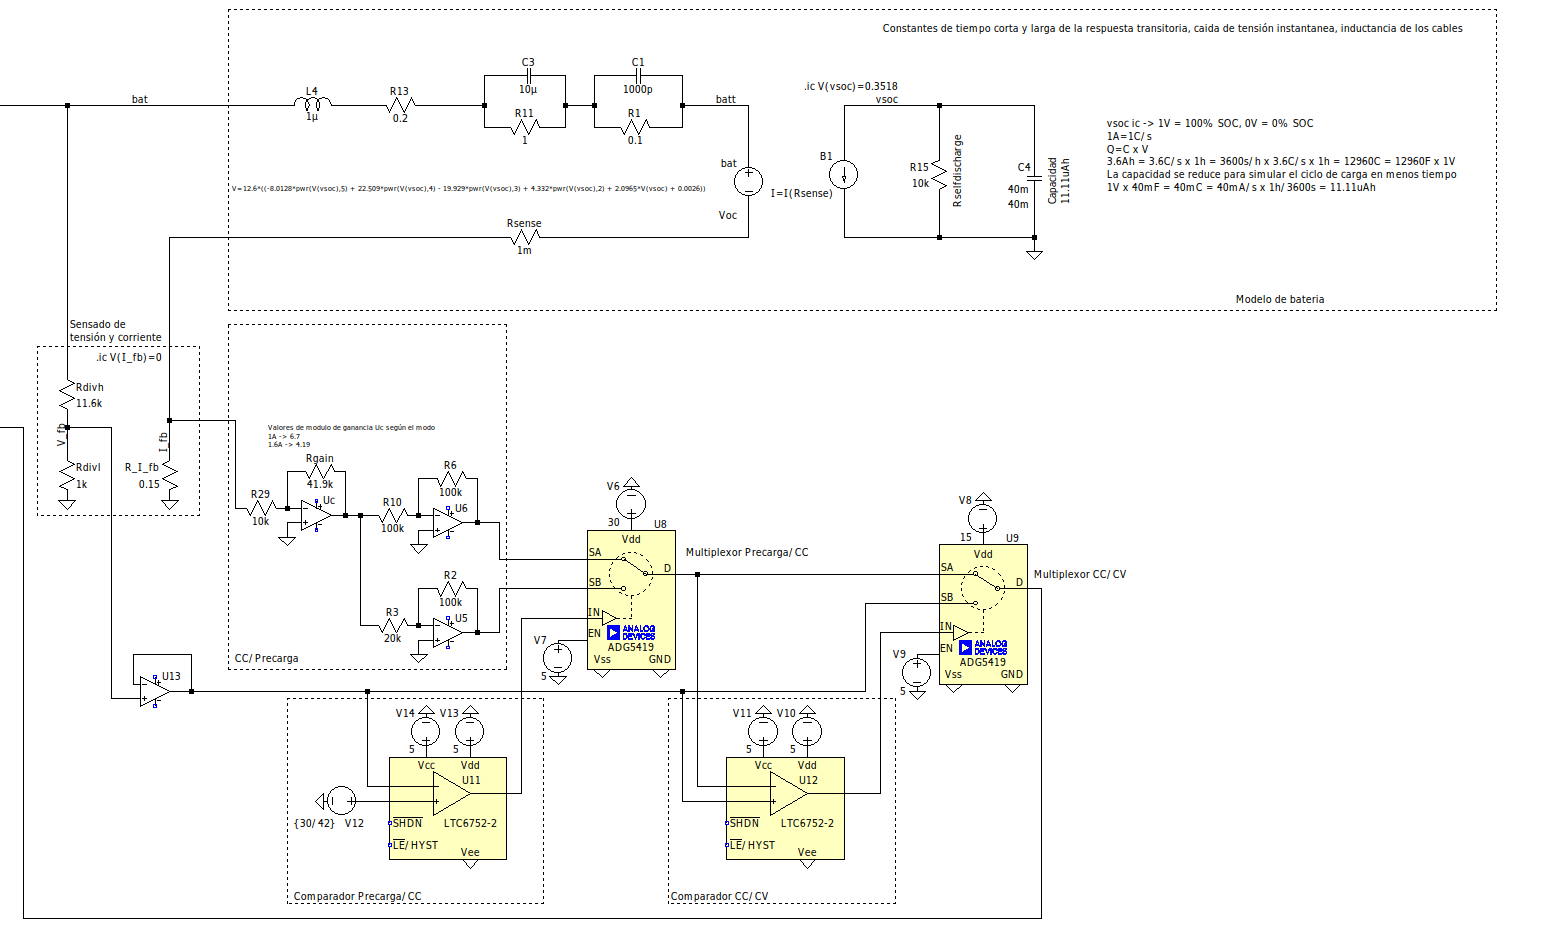
\includegraphics[width=\linewidth]{images/sim-full-2.png}
    \caption{Circuito simulado en LTspice. Se muestra el modelo de batería utilizado y el resto del circuito de control.}
    \label{fig:sim-full-2}
\end{figure}

\begin{figure}[hbt]
    \centering
    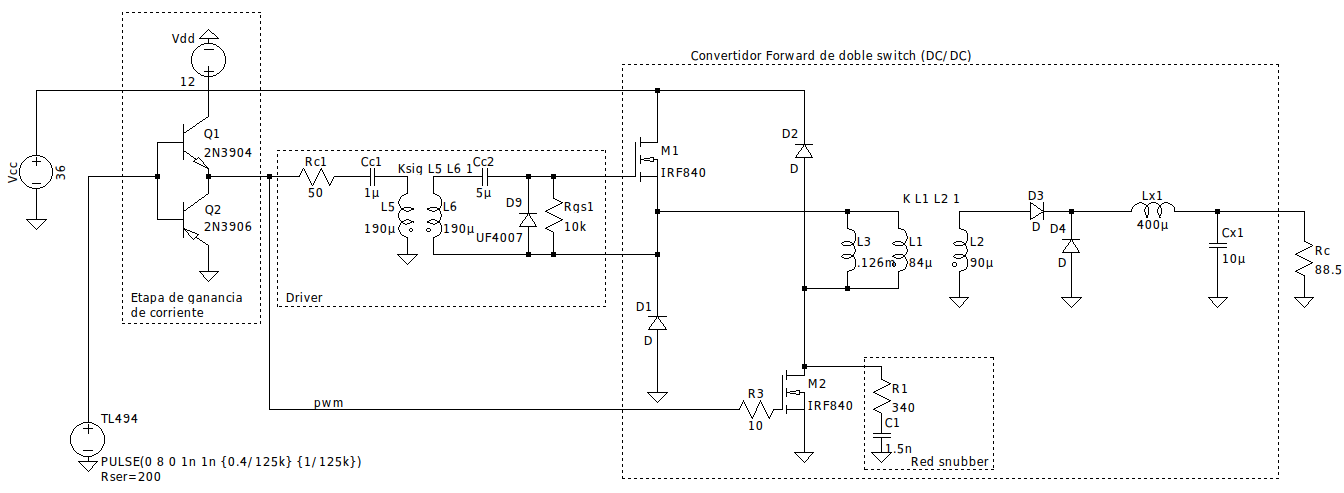
\includegraphics[width=\linewidth]{images/sim-final.png}
    \caption{Circuito final simulado en LTspice}
    \label{fig:sim-final}
\end{figure}

\end{landscape}
\restoregeometry